%!TeX root=../tese.tex

%% ------------------------------------------------------------------------- %%
\chapter{Experimento preliminar}
\label{cap:experimento-preliminar}

Foi realizado um experimento de teste utilizando a nuvem pública de computação
da Amazon Web Services usando uma máquina virtual EC2 com 1 vCPU e 1GB de
memória RAM. Para ter o cenário de um balanceador de carga na frente da
aplicação foi criado um Application Load Balancer direcionando o tráfego
HTTP para esta máquina e coletando os registros das requisições no serviço
de armazenamento S3.

\begin{figure}
  \centering
  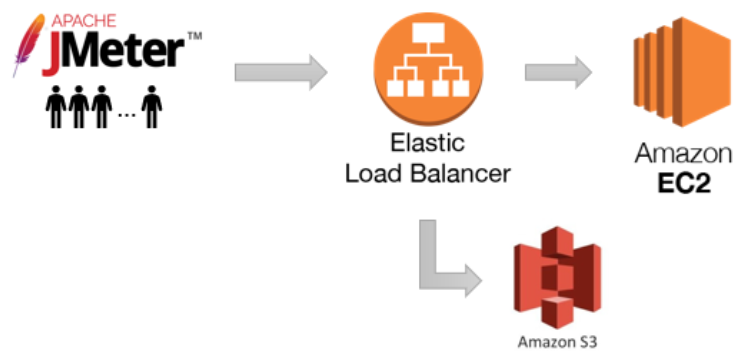
\includegraphics[width=.7\textwidth]{figura9}
  \caption{Diagrama do experimento preliminar.\label{fig:diagrama-do-experimento-preliminar}}
\end{figure}

A aplicação web foi criada utilizando SpringBoot atendendo requisições GET
que executavam o código Java abaixo, consumindo tanto CPU quanto memória:

\begin{program}
  \centering
  \begin{lstlisting}[language=Java, style=wider]
    List<Integer> array = new ArrayList<>();
    for (int index = 0; index < 1000000; index++) {
      array.add((int) (Math.random() * Integer.MAX_VALUE));
    }
    Collections.sort(array);
  \end{lstlisting}
  \caption{Código de teste da aplicação web.\label{prog:java}}
\end{program}

O teste da aplicação foi feito utilizando JMeter para com o número de usuários
concorrentes variando ao longo do tempo chegando a 10 usuários concorrentes.

\begin{figure}
  \centering
  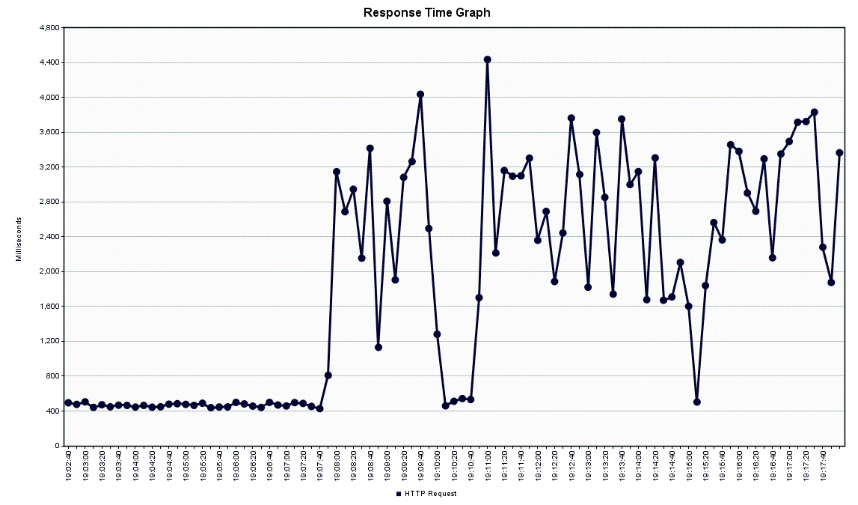
\includegraphics[width=.7\textwidth]{figura10}
  \caption{Tempo de resposta da aplicação ao longo do tempo.\label{fig:tempo-de-resposta-da-aplicação-ao-longo-do-tempo}}
\end{figure}

A figura acima mostra o tempo de resposta da requisição ao longo da execução
do teste. A aplicação se comporta bem no início, porém após os créditos de
CPU da instância se esgotarem ela começa a ter tempos de resposta bastante
altos, e será justamente esta anomalia que desejamos identificar neste
experimento.

Os créditos de CPU mencionados são uma forma da AWS permitir que a máquina
utilize um pouco mais de CPU durante picos de uso, pois créditos de CPU são
incrementados até um certo limite caso a máquina esteja ociosa, ou
consumidos em caso de alta carga.

Foram coletados 565 registros do ALB correspondentes a este teste e algumas
amostras estão nas tabelas abaixo, onde os valores das colunas correspondem a:

\begin{enumerate}
  \item Data e hora do início da requisição no ALB no formato ISO-8601;
  \item Data e hora do término da requisição no ALB no formato ISO-8601;
  \item Instância de destino que executou a requisição;
  \item Tempo de processamento da requisição no destino;
  \item Código de resposta HTTP;
  \item Quantidade de bytes enviados a aplicação;
  \item Quantidade de bytes recebidos da aplicação;
  \item Verbo HTTP utilizado pela requisição;
  \item Caminho da URL utilizado na requisição.
\end{enumerate}

\begin{sidewaystable}[H]
\centering
\caption{Exemplos de registros regulares e anômalos do balanceador de carga.}
Estes exemplos são registros regulares:

\vspace{0.25cm}
\begin{tabular}{lllllllll}
1                           & 2                           & 3                 & 4     & 5   & 6   & 7   & 8   & 9     \\
\hline
2019-11-21T21:02:56.898000Z & 2019-11-21T21:02:57.250351Z & 172.31.7.121:8080 & 0.351 & 200 & 292 & 175 & GET & /test \\
2019-11-21T21:02:57.886000Z & 2019-11-21T21:02:58.233481Z & 172.31.7.121:8080 & 0.347 & 200 & 292 & 175 & GET & /test \\
2019-11-21T21:02:58.877000Z & 2019-11-21T21:02:59.220909Z & 172.31.7.121:8080 & 0.343 & 200 & 292 & 175 & GET & /test \\
2019-11-21T21:02:59.868000Z & 2019-11-21T21:03:00.348951Z & 172.31.7.121:8080 & 0.480 & 200 & 292 & 175 & GET & /test \\
2019-11-21T21:03:00.984000Z & 2019-11-21T21:03:01.337323Z & 172.31.7.121:8080 & 0.352 & 200 & 292 & 175 & GET & /test
\end{tabular}

\vspace{2cm}

Estes exemplos foram considerados anômalos:

\vspace{0.25cm}
\begin{tabular}{lllllllll}
1                           & 2                           & 3                 & 4     & 5   & 6   & 7   & 8   & 9     \\
\hline
2019-11-21T21:16:04.811655Z & 2019-11-21T21:16:00.847000Z & 172.31.7.121:8080 & 3.964 & 200 & 328 & 174 & GET & /test \\
2019-11-21T21:16:09.250483Z & 2019-11-21T21:16:05.195000Z & 172.31.7.121:8080 & 4.054 & 200 & 328 & 174 & GET & /test \\
2019-11-21T21:16:13.374715Z & 2019-11-21T21:16:09.344000Z & 172.31.7.121:8080 & 4.030 & 200 & 328 & 174 & GET & /test \\
2019-11-21T21:16:32.603263Z & 2019-11-21T21:16:28.658000Z & 172.31.7.121:8080 & 3.945 & 200 & 328 & 174 & GET & /test \\
2019-11-21T21:16:51.868990Z & 2019-11-21T21:16:47.794000Z & 172.31.7.121:8080 & 4.074 & 200 & 328 & 174 & GET & /test
\end{tabular}
\end{sidewaystable}

Além do aumento no tempo de execução (coluna 3) é possível notar um aumento
discreto no tamanho da quantidade de bytes recebidos, talvez por algum
cabeçalho HTTP adicional, mas ainda não foi investigado o que provocou esta
alteração.

Utilizando os primeiros 300 registros com respostas bem similares para a etapa
de treinamento da distribuição gaussiana multivalorada, marcamos os registros
com menos de 10\% de probabilidade como anômalos e os resultados foram plotados
na figura 5.3.

\begin{figure}
  \centering
  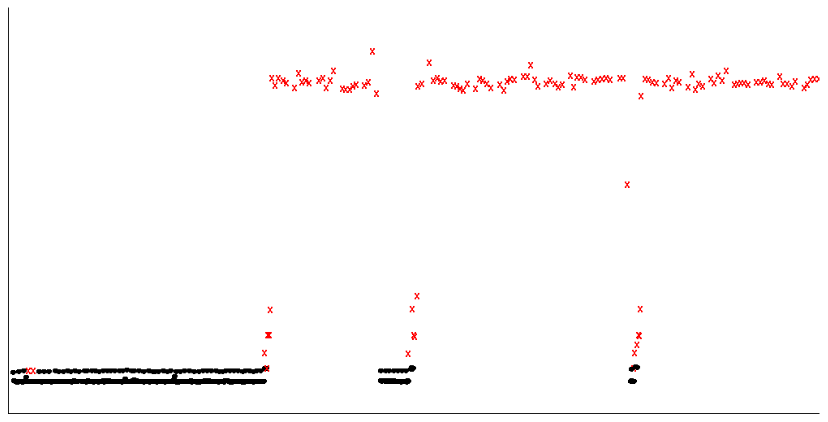
\includegraphics[width=.7\textwidth]{figura11}
  \caption{Anomalias detectadas no experimento.\label{fig:anomalias-detectadas-no-experimento}}
\end{figure}

É possível ver que a classificação de anomalia funciona bem neste cenário controlado
e que alguns registros que deveriam ser considerados normais foram marcados como
anômalos.

Logo no começo é possível ver dois pontos vermelhos que representam duas amostras
que levaram o tempo de 483 e 488 milissegundos enquanto a carga da aplicação
percebida era de 1 execução concorrente. O tempo médio de resposta no
treinamento era de 375 milissegundos e dada a pouca variação ocorrida nos
primeiros 300 registros estes tempos foram marcados como anormais.

Pouco antes de começarem a ocorrer várias falhas com tempos bastante altos foi
detectado um registros com 514 milissegundos de execução. Como a informação de
carga era de que haviam duas execuções concorrentes neste instante a requisição
foi marcada como normal.
 
Com esta observação é possível afirmar que a informação de carga na aplicação estava
de fato sendo considerada na detecção de anomalia, pois a requisição que levou 483
milissegundos no início do teste (sem concorrência) foi identificada como anômala.
